\chapter{State of the art} \label{chap:state_of_the_art}
Om de achtergrond te schetsen waarbinnen het werk van deze thesis besproken kan worden, onderscheiden we twee grote stromingen: het Android besturingssysteem en locatieverzameling/-obfuscatie. Ook is er een extra sectie voorzien voor het onderzoek naar hoe de standaardimplementatie van obfuscatie werkt in Android want de documentatie bespreekt sommige dingen niet.
\section{Android besturingssysteem}
\subsection{Library}
Omdat ontwikkelaars een code efficiënt zouden kunnen implementeren zonder herhaaldelijk gebruik te maken van copy-paste, worden libraries gebruikt. Android-applicaties worden voornamelijk geprogrammeerd in Java of Kotlin, waarbij de build-tool Gradle wordt ingezet. Deze build-tool beheert de installatie van de benodigde libraries, zodat deze eenvoudig beschikbaar zijn voor integratie in de eigen code.
In tegenstelling tot een standaard applicatie, die wordt gecompileerd naar een \gls{apk}, wordt een library voor Android gecompileerd naar een \gls{aar}.

Deze \gls{aar}-bestanden kunnen vervolgens worden gepubliceerd naar publieke Gradle-plugins, waardoor ze eenvoudig herbruikbaar zijn in andere projecten door deze te importeren.
\subsection{Activity}
Een activity in Android is een enkele, gefocuste taak die een gebruiker kan uitvoeren. Het vormt een van de fundamentele bouwstenen van een Android-applicatie. Elke activity heeft een eigen lifecycle, die wordt beheerd door het Android-systeem. Deze lifecycle bestaat uit verschillende states.

Elke state-overgang heeft ook een methode zoals onCreate, onStart, onResume, onPause, onStop en onDestroy. Die de ontwikkelaar kan overschrijven om zo de overgang beter te kunnen afhandelen.

Bij het ontwikkelen van een applicatie is het belangrijk om rekening te houden met deze lifecycle-methoden, omdat ze bepalen hoe de applicatie reageert op gebruikersinteracties en systeemgebeurtenissen. Bijvoorbeeld, in de onCreate-methode wordt de initiële setup van de activity uitgevoerd, zoals het instellen van de gebruikersinterface. De onPause- en onStop-methoden worden aangeroepen wanneer de activity naar de achtergrond gaat, en resources kunnen hier worden vrijgegeven om geheugen te besparen.

Zo heeft elke state bepaalde eigenschappen. Zo worden langdurige taken die in de states draaien, waarbij de activity naar de achtergrond gaat, abrupt gestopt als het systeem resources nodig heeft en is dus niet vertrouwbaar. Om dit probleem te omzeilen biedt Android alternatieve oplossingen zoals services(waarover sectie hoofdstuk meer).
Daarnaast is het niet toegestaan om blocking calls, zoals een HTTP-request of het opvragen van locatiegegevens via de Location Provider, uit te voeren in de main thread. Dit is noodzakelijk om te voorkomen dat de gebruikersinterface vastloopt en de gebruikservaring negatief wordt beïnvloed. Zo crashed de applicatie als de main thread wordt geblocked voor meer dan vijf seconden.
\begin{figure}[h]
    \centering
    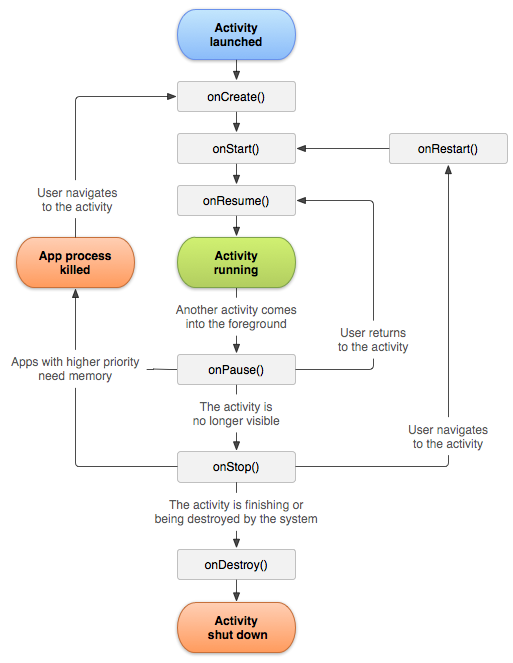
\includegraphics[width=0.75\textwidth]{images/activity_lifecycle.png}
    \caption{Activity lifecycle Android\cite{android_activity}}
    \label{fig:android_lifecycle}
\end{figure}
\subsection{Achtergrondwerk }
\begin{figure}
    \centering
    \includesvg[width=0.75\textwidth]{images/event-tasks-flowchart.svg}
    \caption{Keuze boom achtergrondwerk voor event driven tasks \cite{android_background_work}}
    \label{fig:android_background_work}
\end{figure}
Om de hierboven vermelde beperkingen van een activity, die slechts kort op de achtergrond actief kan blijven, te omzeilen. Biedt Android verschillende tools die door de jaren heen zijn geëvolueerd. Deze tools maken het mogelijk om taken los van de activity uit te voeren, zelfs wanneer de applicatie niet actief is.
Maar elke \gls{api} is verschillend om zo elk soort probleem aan te pakken. Hier focussen we op de keuze boom gerelateerd voor het starten van een achtergrond taak gebaseerd op een event. Dit omdat de optie om een eenmalige locatie op te vragen in de applicatie kan afgehandeld worden door een simpele thread.

Zoals te zien in Figuur~\ref{fig:android_background_work} is asynchrone werk niet van toepassing voor deze thesis omdat het over langdurige verzameling gaat. Dan heb je nog Task scheduling en Foreground services. Hierin zijn de belangrijkste tools zijn de AlarmManager en  de WorkManager. 
\paragraph{AlarmManager}\cite{android_alarmmanager}
Alarm manager is een implementatie van een task scheduling \gls{api}
De AlarmManager is een mechanisme dat het apparaat uit de zogenaamde 'doze mode' of energiebesparende modus kan halen. Dit maakt het mogelijk om op specifieke tijdstippen een taak uit te voeren. Echter, de AlarmManager heeft enkele beperkingen. Zo kan het slechts één keer per uur een taak uitvoeren en is het niet geschikt voor langdurige taken. Dit maakt het minder geschikt voor toepassingen die continu of frequent achtergrondtaken moeten uitvoeren.
AlarmManager wordt dikwijls gebruikt om persistent achtergrondwerk op te starten als de applicatie niet opgestart is.

\paragraph{WorkManager}\cite{android_persistent}
De WorkManager is een krachtig en flexibel \gls{api} voor het uitvoeren van taken die niet gekoppeld zijn aan een activity. 
Het is zowel een oplossing voor foreground services als voor task scheduling. 
Zo biedt ondersteuning voor zowel eenmalige langdurige (one-time) als periodieke (periodic) taken. Voor achtergrondtaken die regelmatig moeten worden uitgevoerd, zoals het verzamelen van locatiegegevens, is de periodieke versie geschikt. 

Hierbij kan een taak bijvoorbeeld elke 15 minuten worden uitgevoerd, met een maximale duur van 10 minuten per taak. 
Voor taken die slechts één keer hoeven te worden uitgevoerd, al dan niet langdurig, kan de eenmalige versie worden gebruikt. Het is echter een belangrijk punt om op te merken dat langdurige taken in de foreground moeten lopen. Dit betekent dat er een permanente notificatie zichtbaar moet zijn, wat de gebruiker kan storen.

\begin{figure}[h]
    \centering
    \includesvg[width=0.75\textwidth]{images/workmanager_main.svg}
    \caption{Android WorkManager}
    \label{fig:workmanager}
\end{figure}
\paragraph{Coroutines}\cite{kotlin_coroutines}
Coroutines vormen geen \gls{api} voor het aanbieden van persistente services, maar zijn wel de aangewezen oplossing voor het uitvoeren van zware of blocking taken buiten de hoofdthread van een activity. Coroutines kunnen worden beschouwd als lichtgewicht alternatieven voor threads en bieden een efficiënte manier om asynchrone taken uit te voeren zonder de gebruikersinterface te blokkeren. Ze zijn echter gekoppeld aan de lifecycle van de aanroepende component (zoals een activity of fragment). Dit betekent dat wanneer de activity wordt gestopt, ook de bijbehorende coroutines worden beëindigd. Hierdoor zijn coroutines niet geschikt voor persistent achtergrondwerk dat moet blijven draaien, ongeacht de status van de activity.
Dit zou dus een oplossing kunnen zijn om eenmalige een locatie op te vragen.
\section{Locatie obfuscatie}
In de studie van obfuscatie heb je 2 paden: hoe Android het aanpakt en voorgaand onderzoek losstaand van Android.
\subsection{Android's oplossing}
Voordat er dieper wordt ingegaan op locatie-obfuscatie in Android, is het belangrijk om de werking van de locatievoorzieningen in Android te bespreken. Android biedt twee primaire opties om locatiegegevens op te vragen: de standaard open-source implementatie en de Google Play Services-implementatie.

De standaard open-source implementatie leest enkel de data uit van de sensoren en voert geen verdere berekeningen of obfuscatie-algoritmes uit. Deze aanpak biedt ontwikkelaars meer vrijheid, maar brengt ook enkele nadelen met zich mee. Zo worden applicaties die deze versie gebruiken vaker gemarkeerd als potentieel kwaadaardig, omdat ze minder geïntegreerd zijn in het Google Android-ecosysteem.

De Google Play Services-implementatie, daarentegen, maakt gebruik van de Fused Location Provider. De Fused Location Provider combineert gegevens van verschillende sensoren, zoals \gls{gps}, wifi, mobiele netwerken en zelfs bewegingssensoren, om een zo nauwkeurig mogelijke locatie te berekenen. Dit proces wordt \"sensor fusion\" genoemd. De Fused Location Provider biedt ontwikkelaars een \gls{api} om locatiegegevens op te vragen, waarbij automatisch de meest geschikte bron wordt gekozen op basis van de context, zoals batterijverbruik, nauwkeurigheid en beschikbaarheid van sensoren. Bovendien ondersteunt de Fused Location Provider zowel real-time locatie-updates als eenmalige locatieverzoeken, wat het een flexibele oplossing maakt voor uiteenlopende toepassingen.

In de Fused Location Provider zijn er verschillende parameters om locatiegegevens te verkrijgen. 
De meest nauwkeurige methode gebruikt alle sensoren inclusief \gls{gps}-satellieten, maar alternatieve methoden zoals enkel het gebruik van lokale telefoonmasten en wifi-netwerken is ook een mogelijkheid. 
Deze alternatieve methoden introduceren een inherente vorm van obfuscatie, aangezien de nauwkeurigheid doorgaans lager is dan die van \gls{gps}. Echter, in dichtbevolkte stedelijke gebieden kan dit juist leiden tot een hogere nauwkeurigheid dan \gls{gps}, omdat gebouwen \gls{gps}-signalen kunnen blokkeren.

Verder nog, sinds Android 12 hebben gebruikers de mogelijkheid gekregen om alleen toegang tot een benaderde locatie (approximate location) toe te staan, wat een extra dimensie toevoegt aan de discussie over privacy en nauwkeurigheid.
De coarse location-functionaliteit in Android maakt geen gebruik van \gls{gps}-satellieten en voegt bovendien een extra laag van obfuscatie toe aan de locatiegegevens. Hoe deze obfuscatie precies wordt toegepast, is echter niet publiekelijk gedocumenteerd. Door dit zijn er preliminaire onderzoeken uitgevoerd waarover later meer.

\subsection{Voorgaand onderzoek}
Naast de oplossing van Android en nog voor Android 12 werd er al onderzoek gedaan naar de mogelijke gevaren en oplossingen.
\paragraph{Aanval van Kevin De Boeck} \cite{kevin}
In eerdere onderzoeken, uitgevoerd door Kevin De Boeck, werd aangetoond dat locatie-obfuscatie een dringende noodzaak is. Uit data-analyse op een dataset van locatiegegevens in Frankrijk, verzameld over een periode van een week, bleek dat gevoelige locaties eenvoudig konden worden geïdentificeerd. Denk maar aan als er 50 punten op een heel afgelegen plek liggen dat dit misschien een overheids instelling kan zijn dat geheim moet blijven.
Ook op vlak van het individu kon makkelijk een thuis of andere persoonlijke locaties gevonden worden. Verder konden er sociale grafen gemaakt worden en zelfs een volledige vakantie reis in kaart gebracht worden.

\paragraph{Oplossing Toon Dehaene} \cite{DehaeneToon2023MLSi}
Voortbouwend op deze bevindingen heeft Toon Dehaene onderzoek gedaan naar methoden om \gls{gps}-locaties te obfusceren.
Hiervoor werd een library ontwikkeld in Rust met behulp van PyO3, zodat deze als Python-module kon worden gebruikt voor het verwerken van grote datasets. Het doel was om locatie-traces op serverzijde te obfusceren. Naast de implementatie van parallellisatie was het kernalgoritme voor obfuscatie als volgt:
\begin{itemize}
    \item Wanneer er onvoldoende tijd is verstreken sinds de vorige locatie, wordt simpelweg de vorige locatie opnieuw doorgestuurd.
    \item Vervolgens wordt het concept van privacycirkels toegepast: als de nieuwe locatie binnen een bestaande privacycirkel valt, wordt het middelpunt van deze cirkel samen met de huidige tijdstempel doorgestuurd. 
    \item Valt de locatie buiten alle bestaande cirkels, dan wordt er een nieuwe cirkel aangemaakt met een willekeurige hoek en een straal die willekeurig gekozen wordt tussen 0 en de huidige maximale straal. De gebruiker valt dan altijd binnen deze nieuw gegenereerde cirkel, waarvan het middelpunt wordt doorgestuurd.
\end{itemize}

Dit algoritme introduceert dus ruis op de coördinaten en, belangrijker nog, voorkomt dat derden door het nemen van gemiddelden van geobfusceerde locaties alsnog gevoelige locaties kunnen achterhalen. Het algoritme vormde tevens de basis voor de standaardimplementatie van obfuscatie in de Android-library, wat verderop wordt toegelicht. Dit omdat dit algoritme uiterst geschikt is voor real-time data obfuscatie, waar als andere obfuscatie-methoden alle data op voorhand nodig hebben.
\paragraph{Testen van de oplossing}
In verder onderzoek van Toon Dehaene werd nagegaan of deze geobfusceerde locaties konden worden teruggevonden via gridsnapping. 
Dit werd onderzocht om de effectiviteit van locatieobfuscatie in afgelegen gebieden te evalueren. Wanneer er zich slechts één straat binnen de straal van een privacycirkel bevindt, is het immers visueel eenvoudig om de oorspronkelijke route te reconstrueren. (Dit roept de vraag op of de straal van de privacycirkel dynamisch zou moeten worden aangepast op basis van de bebouwingsdichtheid.)

Een bijkomende onderzoeksvraag was of het mogelijk is om een obfuscatiemethode te ontwikkelen waarbij de geobfusceerde locatie bewust op een willekeurige, maar plausibele locatie binnen een grid wordt geplaatst, zodat de geobfusceerde locaties in afgelegen gebieden realistischer lijken. Uit de resultaten bleek echter dat deze aanpak een averechts effect had. Verder onderzoek naar deze methode valt buiten de scope van deze thesis.

\section{Preliminaire experimenten}
Aangezien de Android Developer-website niet alle vragen beantwoorde en er nog veel onduidelijkheden zijn, is een deel van de state-of-the-art gewijd aan onderzoek naar hoe deze variabelen het uiteindelijke resultaat beïnvloeden.
\subsection{Verschillende nauwkeurigheidsniveaus}
De Fused Location Provider biedt vier prioriteitsniveaus voor het bepalen van de locatie, zoals beschreven in de Android-documentatie \cite{location_battery}:

\begin{itemize}
    \item \textbf{Balanced power accuracy}: Gebruik deze instelling om locatieprecisie op te vragen binnen een stadsblok, wat een nauwkeurigheid van ongeveer 100 meter is. Dit wordt beschouwd als een grove nauwkeurigheid en verbruikt waarschijnlijk minder stroom. Met deze instelling maken de locatieservices waarschijnlijk gebruik van Wi-Fi en positionering van zendmasten. Houd er echter rekening mee dat de keuze van de locatieprovider afhankelijk is van veel andere factoren, zoals welke bronnen beschikbaar zijn.
    \item \textbf{High accuracy}: Gebruik deze instelling om de meest nauwkeurige locatie op te vragen. Met deze instelling is de kans groter dat de locatieservices \gls{gps} gebruiken om de locatie te bepalen.
    \item \textbf{Low power}: Gebruik deze instelling om precisie op stadsniveau aan te vragen, wat een nauwkeurigheid van ongeveer 10 kilometer is. Dit wordt beschouwd als een grove nauwkeurigheid en verbruikt waarschijnlijk minder stroom.
    \item \textbf{Passive}: Gebruik deze instelling als u een verwaarloosbare invloed op het stroomverbruik nodig heeft, maar locatie-updates wilt ontvangen wanneer deze beschikbaar zijn. Met deze instelling activeert uw app geen locatie-updates, maar ontvangt u locaties die door andere apps worden geactiveerd.
\end{itemize}

Naast de beschreven verschillen in nauwkeurigheid en energieverbruik, zijn er ook andere factoren die deze instellingen beïnvloeden. Uit experimenten bleek bijvoorbeeld dat de instelling \textit{balanced power accuracy} wordt beïnvloed door de doze-modus of energiebesparingsmodus van Android. Tijdens tests werd vastgesteld dat een actief gebruikte telefoon een consistente locatie-trace genereerde, terwijl drie andere telefoons aanzienlijke hiaten vertoonden. Deze hiaten werden veroorzaakt doordat de Fused Location Provider de callback niet activeerde vanwege de energiebesparende staten.

Tests met de prioriteiten \textit{low power} en \textit{passive} werden niet uitgevoerd. De \textit{low power}-instelling was niet relevant voor onderzoek naar gebruikerslocatie-traces. Dit doordat de beloofde nauwkeurigheid 10km is. De \textit{passive}-instelling niet omdat er te veel externe variabelen zijn, waardoor geen waardevolle resultaten konden worden verkregen.
In voornaamste omdat de locatieupdates afhankelijk zijn van wat andere applicaties doen.

\subsection{Coarse location Android}
Om de coarse location-functionaliteit te onderzoeken, werd de applicatie tweemaal geïnstalleerd op dezelfde telefoon: één keer met coarse location-permissies en één keer met fine location-permissies. Beide applicaties waren geconfigureerd met dezelfde prioriteitsinstellingen om een eerlijke vergelijking mogelijk te maken. Een van de vragen was of de instelling \textit{balanced power accuracy}, die geen gebruik maakt van satellieten, dezelfde resultaten zou opleveren als coarse location. 
Dit zou inzicht geven in de vraag of de obfuscatie uitsluitend voortkomt uit de inherente onnauwkeurigheid van de gebruikte technologieën, of dat Android actief een extra laag van obfuscatie toepast op de locatiegegevens.
Als resultaat vinden we de volgende visualisatie Figuur~\ref{fig:coarsevsfine1} en Figuur~\ref{fig:coarsevsfine2}. Hierbij is rood de trace met fine permissies en blauw coarse permissies. 
\begin{itemize}
    \item In beide voorbeelden zien we dat de coarse trace duidelijk minder punten bevat en verder van de werkelijke trace ligt dan de fine trace. Dit komt doordat, wanneer de nieuwe locatie te dicht bij de vorige ligt, de callback eenvoudigweg niet wordt opgeroepen.
    \item In het tweede voorbeeld zien we dat bij langdurig op dezelfde locatie blijven, de fine permissie relatief veel punten oplevert, waarbij de data varieert en zelfs een uitschieter vertoont. Dit is waarschijnlijk het gevolg van meer interferentie op de signalen in een betonnen gebouw. Opvallend is dat wanneer deze uitschieter optreedt, de coarse locatie eveneens een uitschieter in dezelfde richting vertoont. In dat geval wordt de callback dus wel opgeroepen.
    \item In het eerste voorbeeld zien we dat het coarse pad slechts vijf punten bevat. Ook ligt het pad meer dan de helft van de breedte van Gent verwijderd van de werkelijke trace. De obfuscatie-oplossing van Android kan niet beïnvloed worden door de gebruiker noch developer.
    \item In het tweede voorbeeld zien we linksboven op de Gentse Steenweg bij de Colruyt dat, wanneer er een volgend punt wordt berekend door de coarse-methode, dit punt ver genoeg van de vorige punten ligt. Dit kan mogelijk een extra privacymaatregel zijn.
\end{itemize}
Uit deze bemerkingen kunnen we concluderen dat bovenop de inherente onnauwkeurigheid ook nog extra obfuscatie gebeurd.
\begin{figure}[h]
    \centering
    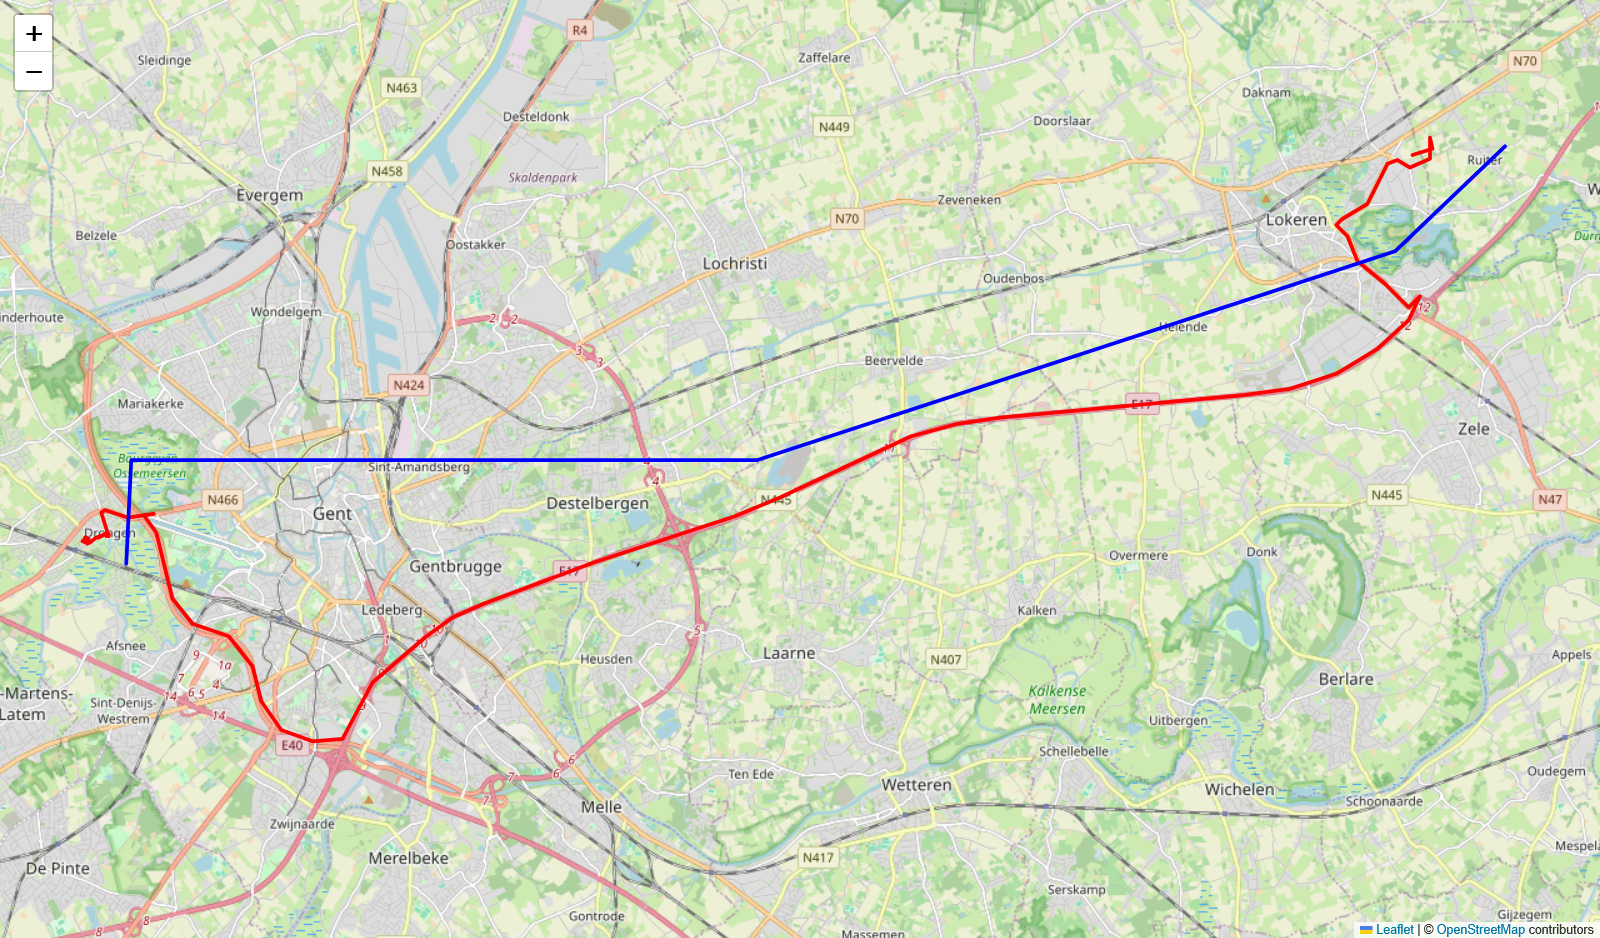
\includegraphics[width=\textwidth]{images/coarsevsfine1.png}
    \caption{Vergelijking coarse permissies en fine permissies 1}
    \label{fig:coarsevsfine1}
\end{figure}
\begin{figure}[h]
    \centering
    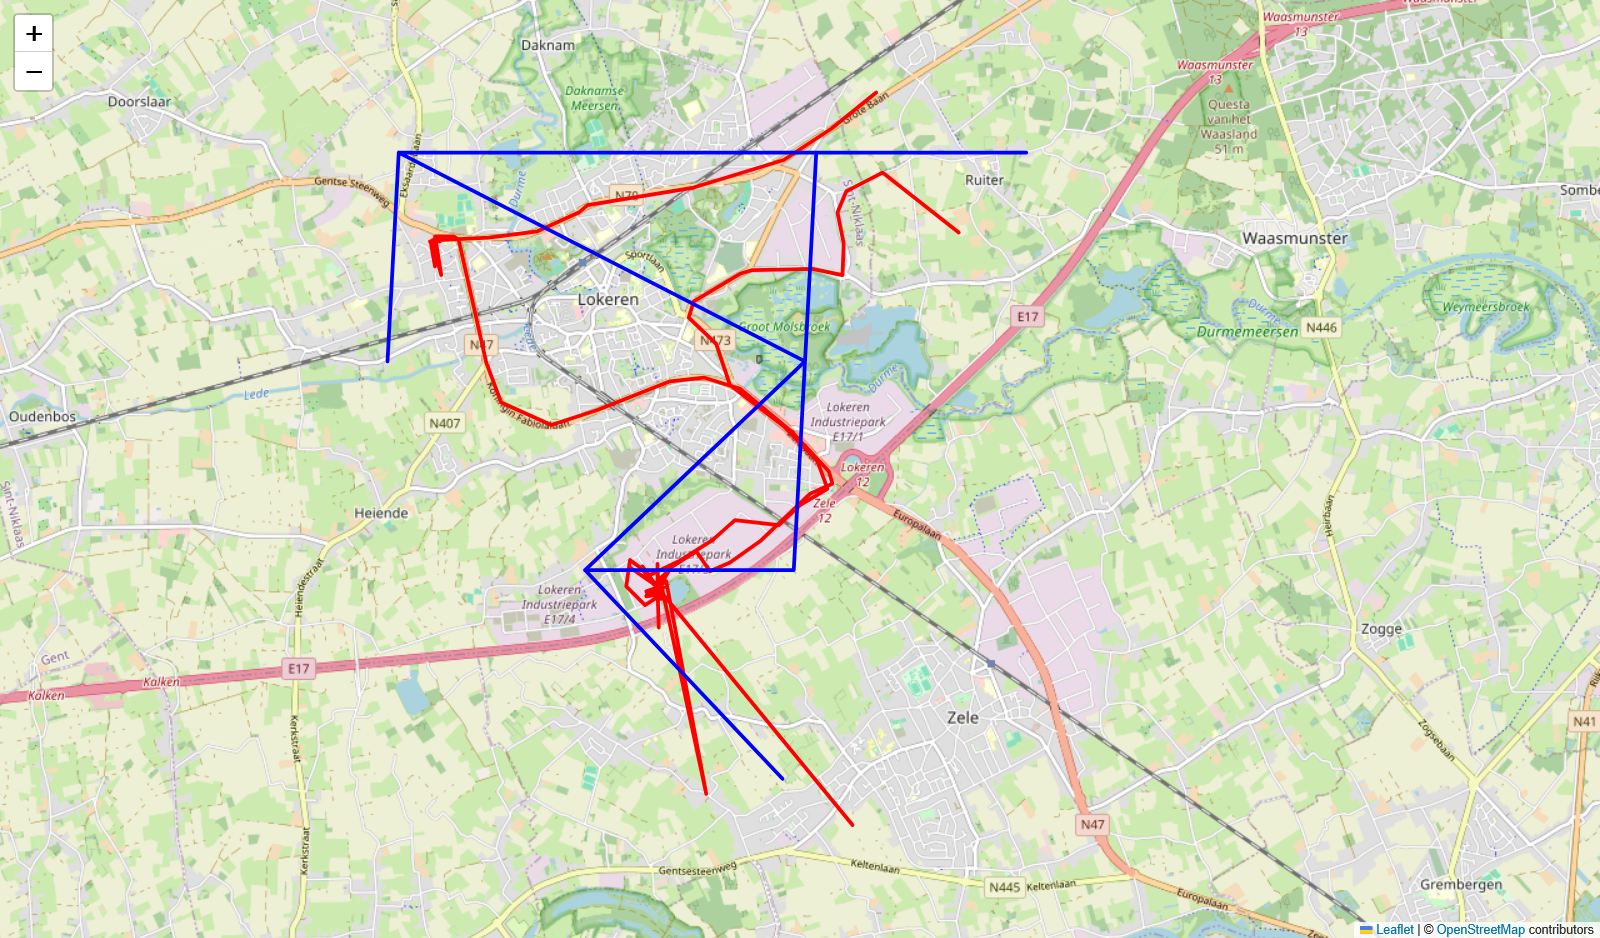
\includegraphics[width=\textwidth]{images/coarsevsfine2.png}
    \caption{Vergelijking coarse permissies en fine permissies 2}
    \label{fig:coarsevsfine2}
\end{figure}
\newline
Een interessante vraag die voortkwam uit deze experimenten, was hoe de obfuscatie van Android precies werkt. Om dit te onderzoeken, werden de coarse location-gegevens van eerdere tests naast elkaar gelegd. 
Zoals te zien is in Figuur~\ref{fig:coarse_1_phone}, leveren de traces van op verschillende dagen maar wel hetzelfde apparaat steeds dezelfde coördinaten op. Dit wijst erop dat Android een soort privacycirkels implementeert, vergelijkbaar met eerder besproken algoritmes, om aanvallen te voorkomen waarbij gemiddelden over lange periodes worden gebruikt om gevoelige locaties te identificeren.

Een vervolgonderzoek richtte zich op de consistentie van dit algoritme. De vraag was of de geobfusceerde locaties consistent worden berekend op basis van nabijgelegen telefoonmasten, zodat dezelfde locaties op verschillende apparaten identiek zouden zijn. Uit de resultaten, weergegeven in Figuur~\ref{fig:coarse_3_phones}, blijkt echter dat dit niet het geval is. Dit suggereert dat Android's obfuscatie-algoritme niet uitsluitend gebaseerd is op vaste berekeningen van telefoonmastlocaties, maar mogelijk ook andere factoren in overweging neemt.
\begin{figure}[h]
    \centering
    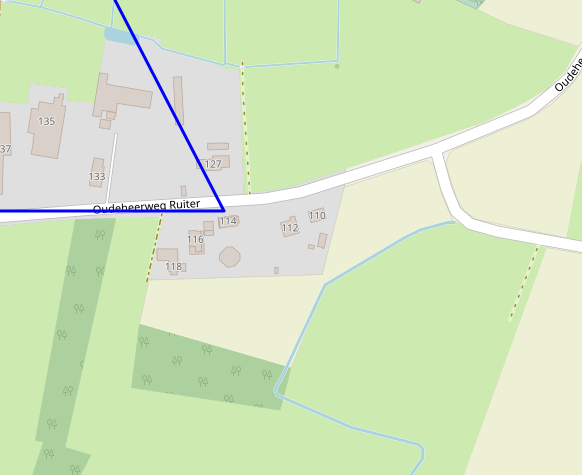
\includegraphics[width=0.24\textwidth]{images/coarse-10-04.png}
    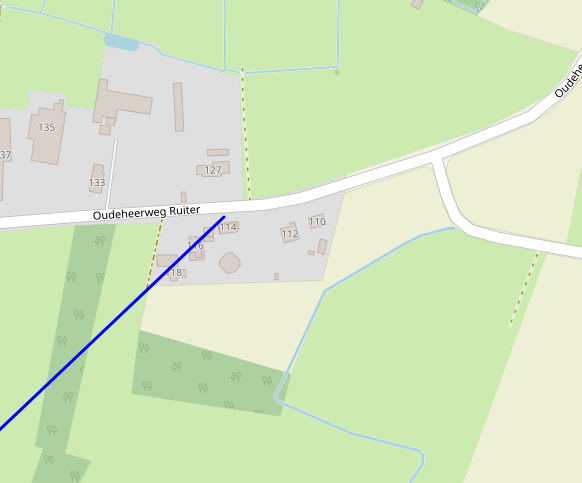
\includegraphics[width=0.24\textwidth]{images/coarse-10-05.png}
    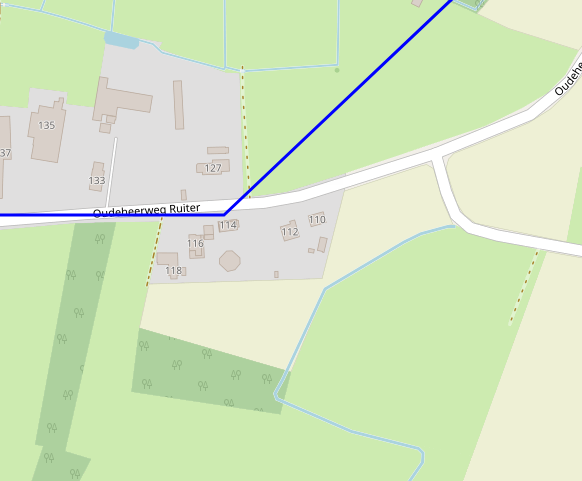
\includegraphics[width=0.24\textwidth]{images/coarse-10-06.png}
    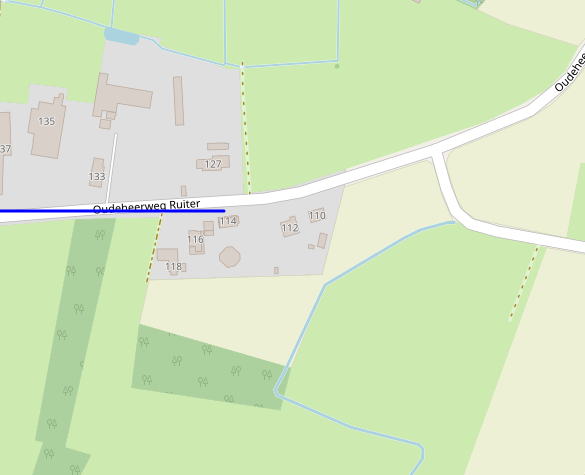
\includegraphics[width=0.24\textwidth]{images/coarse-10-07.png}
    \caption{Vergelijking coarse permissie op één apparaat}\label{fig:coarse_1_phone}
\end{figure}
\begin{figure}[h]
    \centering
    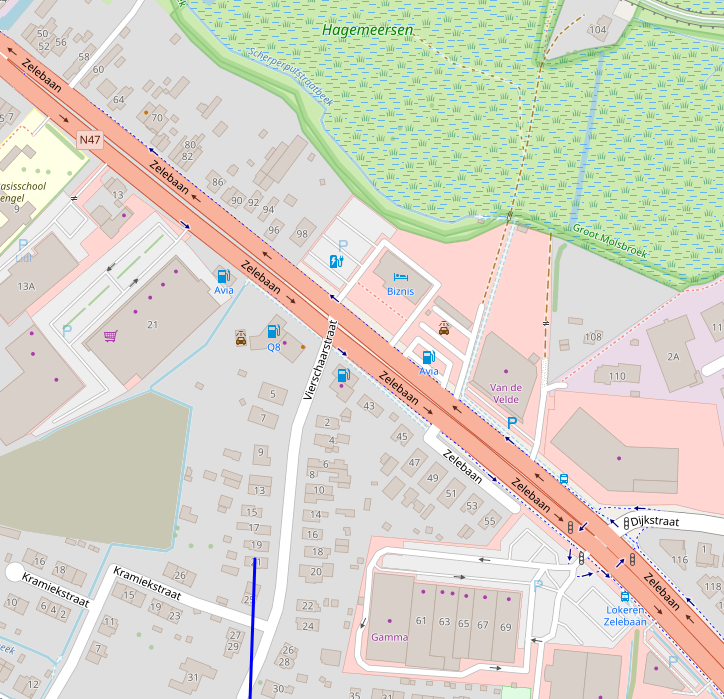
\includegraphics[width=0.32\textwidth]{images/coarse-b76cb5235efc9519.png}
    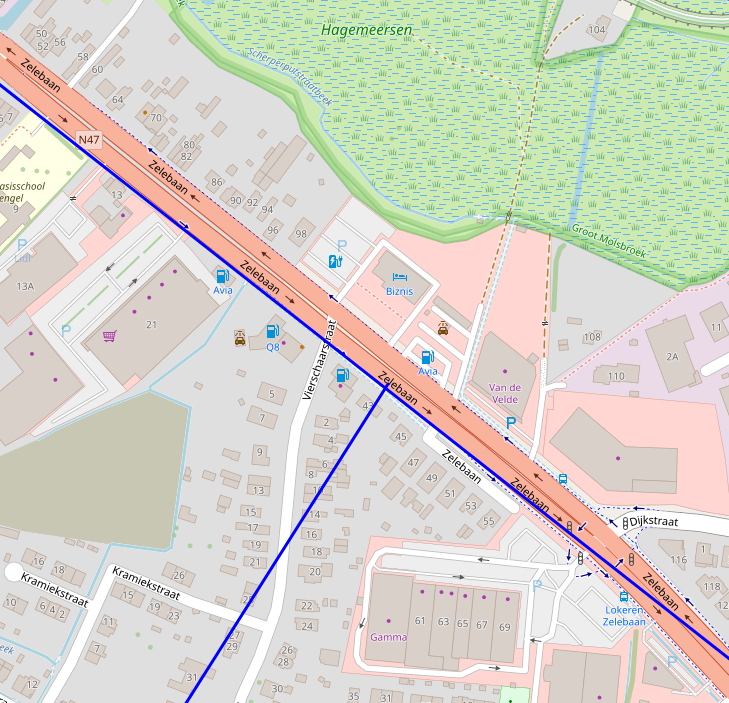
\includegraphics[width=0.32\textwidth]{images/coarse-df4294d41666d9a7.png}
    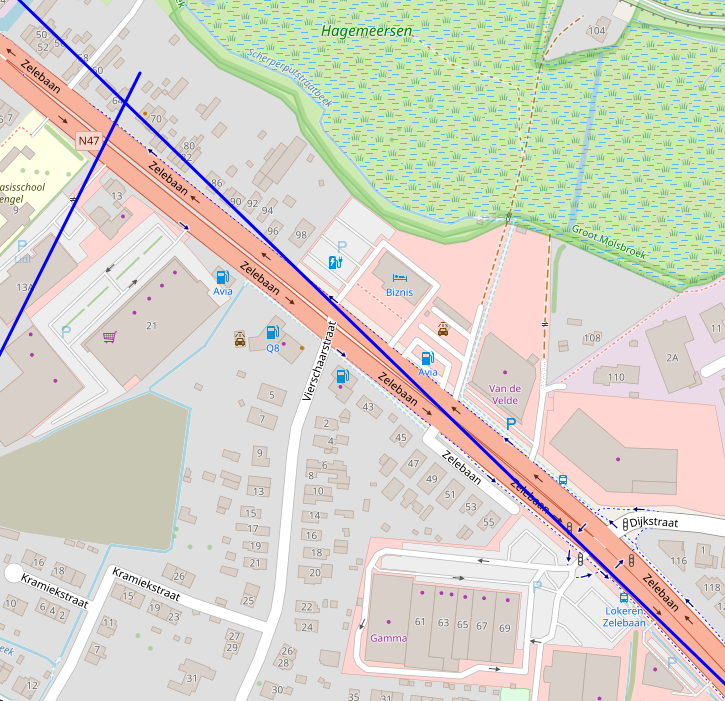
\includegraphics[width=0.32\textwidth]{images/coarse-e41a59c48d43c93e.png}
    \caption{Vergelijking coarse permissie op meerdere apparaten}\label{fig:coarse_3_phones}
\end{figure}
 